\lab{ARMA Models}{ARMA Models}
\label{lab:arma}
\objective{ARMA$(p,q)$ models combine autoregressive and moving-average models in order to forecast future observations using time-series. In this lab, we will build an ARMA$(p,q)$ model to analyze and predict future weather data and then compare this model to statsmodels built-in ARMA package. Then we will forecast the future height of the Rio Negro.}

% spec file should be consistent with std and sigma...change variable to filename
% change from op.fmin to fmin
% change so its ARMA(p,q) in model identification
\section*{Time Series}

A time series is any discrete-time stochastic process.  
In other words, it is a sequence of random variables, $\{y_t\}_{t=1}^n$, that are determined by their time $t$.  
Examples of time series include heart rate readings over time, pollution readings over time, stock prices at the closing of each day, and air temperature.
Often when analyzing time series, we want to forecast future data, such as what will the stock price of a company be in a week and what will the temperature be in 10 days.

\section*{ARMA$(p,q)$ Models}

One way to forecast a time series is using an ARMA model.
An $\text{ARMA}(p,q)$ model combines an autoregressive model of order $p$ and a moving average model of order $q$ on a time series $\{y_t\}_{t = 1}^n$.
This model is a dependent model as it is non-independent of previous data.
Because of this, the model needs to become stationary in order to compensate for the dependency of the data.
To make data stationary, we look at the time series $\{z_t\}_{t=1}^n$ where $z_t=y_t-y_{t-1}$.
The model itself is a stochastic process on $z_t$, satisfying the equation

\begin{align}
    \label{eq:arma:def}
    z_t =\underbrace{\left(\sum_{i=1}^p \phi_{i}z_{t - i}\right)}_\text{AR(p)} + \epsilon_t + 
    \underbrace{\left(\sum_{j=1}^{q} \theta_{j}\epsilon_{t-j} \right)}_\text{MA(q)}
\end{align}
where each $\epsilon_t$ is an identically-distributed Gaussian variable $\mathscr{N}(\mu,\sigma^2),$ and $\phi_i$ and $\theta_j$ are constants.

\subsection*{AR($p$) Models}

An AR($p$) model works similar to a weighted random walk.
Recall that in a random walk, the current position depends on the immediate past position.
In the autogregressive model, the current data point in the time series depends on the past $p$ data points.
However, the importance of each of the past $p$ data points is not uniform.
With an error term to represent white noise and a constant term to adjust the model along the y-axis, we can model the stochastic process with the following equation:

\begin{equation}
z_t=c + \epsilon_t + \sum_{i=1}^p\phi_i z_{t-i}
\label{eq:AR}
\end{equation}

If there is a high correlation between the current and previous values of the time series, then the AR$(p)$ model is a good representation of the data, and thus the ARMA($p,q$) model will most likely be a good representation.
The coefficients $\{\phi_i\}_{i=1}^p$ are larger when the correlation is stronger.

In this lab, we will be using weather data from Provo, Utah\footnote{This data was taken from https://forecast.weather.gov/data/obhistory/metric/KPVU.html}.
To check that the data can be represented well, we need to look at the correlation between the current and previous values.

\begin{figure}[H]
\centering
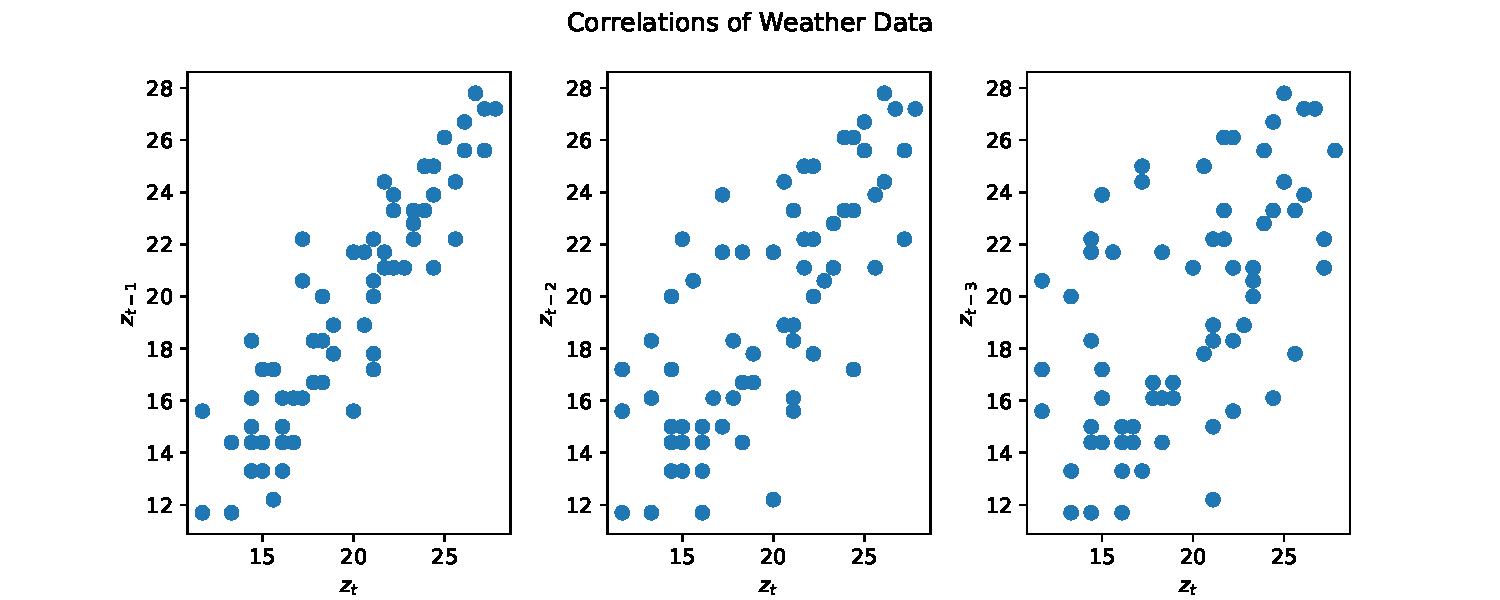
\includegraphics[width=\textwidth]{figures/correlations.pdf}
\caption{These graphs show that the weather data is correlated to its previous values.
The correlation is weaker in each graph successively, showing that the further in the past the data is, the less correlated the data becomes.}
\label{fig:correlations}
\end{figure}

\subsection*{MA($q$)}

A moving average model of order $q$ is used to factor in the varying error of the time series.
This model uses the error of the current data point and the previous data points to predict the next datapoint.
Similar to an AR($p$) model, this model uses a linear combination (which includes a constant term to adjust along the y-axis..

\begin{equation}
z_t = c + \epsilon_t + \sum_{i=1}^q\theta_i\epsilon_{t-i}
\label{eq:MA}
\end{equation}

This part of the model simulates shock effects in the time series.
Examples of shock effects include volatility in the stock market or sudden cold fronts in the temperature.

Combining both the AR$(p$) and MA($q$) models, we get an ARMA($p,q$) model which forecasts based on previous observations and error trends in the data.

\subsection*{Finding Parameters}

One of the most difficult parts of using an ARMA($p,q$) model is identifying the proper parameters of the model.
These parameters include $\{\phi_i\}_{i=1}^p$, $\{\theta_i\}_{i=1}^q$, $\mu$, and $\sigma$, where $\mu$ and $\sigma$ are the mean and variance of the error.
Note that $\{\phi_i\}_{i=1}^p$ and $\{\theta_i\}_{i=1}^q$ determine the order of the ARMA model.

A naive way to use an ARMA model is to choose $p$ and $q$ based on intuition.
Figure \ref{fig:correlations} showed that there is a strong correlation between $z_t$ and $z_{t-1}$ and between $z_t$ and $z_{t-2}$.
The correlation is weaker between $z_t$ and $z_{t-3}$.
Intuition then suggests to choose $p=2$.
By looking at the correlations between the current noise with previous noise, similar to Figure \ref{fig:correlations}, it can also be seen that there is a weak correlation between $z_t$ and $\epsilon_t$ and between $z_t$ and $\epsilon_{t-1}$. 
Between $z_t$ and $\epsilon_{t-2}$ there is no correlation.
For more on how these error correlations were found, see Additional Materials.
Intuition from these correlations suggests to choose $q=1$.
Thus, a naive choice for our model is an ARMA($2,1)$ model.

\begin{figure}[H]
\centering
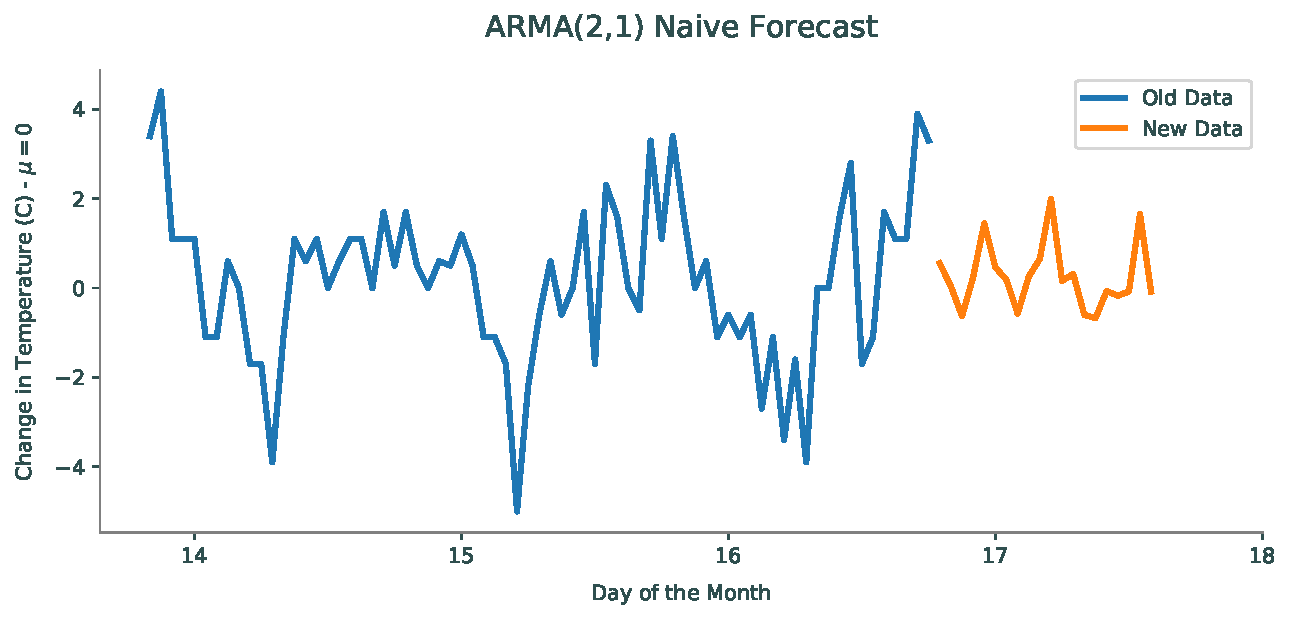
\includegraphics[width=\textwidth]{figures/naive.pdf}
\caption{Naive forecast on \li{weather.npy}}
\label{fig:naive}
\end{figure}

\begin{problem}
Write a function \li{arma_forecast_naive()} that builds an ARMA(p,q) model where the values of $\phi_i=.5$ and $\theta_i=.1$ for all $i$.
Let $\epsilon_i\sim\mathscr{N}(0,1)$ for all $i$.
Use your function to predict the next $n$ values of the time series.
The function should accept a parameter $p$, $q$, and $n$ (the number of observations to predict).
Plot $\{z_t\}_{t=1}^n$ followed by your predicted observations of $z_t$.

The file \li{weather.npy} contains data on the temperature in Provo, Utah from 7:56 PM May 13, 2019 to 6:56 PM May 16, 2019, taken every hour.
Use this file to test your code.
For $p=2$, $q=1$, and $n=20$, your plot should look similar to Figure \ref{fig:naive}, however, due to the variance of the error $\epsilon_t$, the plot will not look exactly like Figure \ref{fig::naive}.
The predictions may be higher or lower on the x-axis.
\label{prob:naive}
\end{problem}

Let $\Theta = \{\phi_i, \theta_j, \mu, \sigma_a^2\}$ be the set of parameters
for an $\text{ARMA}(p,q)$ model. 
Suppose we have a set of observations $\{z_t\}_{t=1}^n$.
Our goal is to find the $p,q$, and $\Theta$ that maximize the likelihood of the ARMA model given the data.
Using the chain rule, we can factorize the likelihood of the model given this data as
\begin{align}
    \label{eq:arma:factorized}
    p(\{z_t\} | \Theta) = \prod_{t=1}^{n} p(z_t | z_{t-1}, \ldots, z_{1},
    \Theta)
\end{align}

\subsubsection*{State Space Representation}

In a general $\text{ARMA}(p,q)$ model, the likelihood is a function of the
unobserved error terms $a_t$ and is not trivial to compute. 
Simple approximations can be made, but these may be inaccurate under certain
circumstances. 
Explicit derivations of the likelihood are possible, but
tedious. 
However, when the $\text{ARMA}$ model is placed in state-space, the
Kalman filter affords a straightforward, recursive way to compute the
likelihood.

We demonstrate one possible state-space representation of an $\text{ARMA}(p,q)$ model. Let
$r = \max(p, q+1)$. Define
\begin{align}
    \hat{\textbf{x}}_{t|t-1}&=\begin{bmatrix}x_{t-1}&x_{t-2}&\dotsb&x_{t-r}\end{bmatrix}^T\\
    F &= \begin{bmatrix}
        \phi_1 & \phi_2 & \cdots & \phi_{r-1} & \phi_r\\
        1 & 0 & \cdots & 0 & 0\\
        0 & 1 & \cdots & 0 & 0\\
        \vdots & \vdots & \cdots & \vdots & \vdots\\
        0 & 0 & \cdots & 1 & 0
    \end{bmatrix}\\
    H &= \begin{bmatrix}
        1 & \theta_1 & \theta_2 & \cdots & \theta_{r-1}
    \end{bmatrix}\\
    Q &= \begin{bmatrix}
        \sigma_a^2 & 0 & \cdots & 0\\
        0 & 0 & \cdots & 0\\
        \vdots & \vdots & \cdots & \vdots\\
        0 & 0 & \cdots & 0
    \end{bmatrix}\\
    w_t &\sim \text{MVN}(0, Q),
    \label{eqn:error}
\end{align}
where $\phi_i = 0$ for $i>p$, and $\theta_j = 0$ for $j > q$. 
Note that Equation \ref{eq:AR} gives
\begin{align}
    F\hat{\textbf{x}}_{t-1|t-2}+w_{t}&=\begin{bmatrix}\sum_{i=1}^r\phi_ix_{t-i}\\
                                x_{t-1}\\
                                x_{t-2}\\
                                \vdots\\
                                x_{t-(r-1)}
                  \end{bmatrix}+\begin{bmatrix}\epsilon_t\\0\\0\\\vdots\\0\end{bmatrix}\\
                &=\begin{bmatrix}x_t&x_{t-1}&\cdots&x_{t-(r-1)}\end{bmatrix}^T\\
                &=\hat{\textbf{x}}_{t|t-1}
\end{align}
We note that $z_{t|t-1}=H\hat{\textbf{x}}_{t|t-1}+\mu$.\footnote{
For a proof of this fact, see Additional Materials.}

Then the linear stochastic
dynamical system
\begin{align}
    \hat{\textbf{x}}_{t+1|t} &= F\hat{\textbf{x}}_{t|t-1} + w_t\\
    z_{t|t-1} &= H\hat{\textbf{x}}_{t|t-1} + \mu
    \label{eq:update-z}
\end{align}
describes the same process as the original $\text{ARMA}$ model.

\begin{info}
Equation \ref{eq:update-z} involves a deterministic component, namely $\mu$.
The Kalman filter theory developed in the previous lab, however, assumed $\mathbb{E}[\epsilon_t]=0$ for the observations $z_{t\mid t-1}$,.
This means you should subtract off the mean
$\mu$ of the error from the time series observations $z_{t\mid t-1}$ when using them in the predict and update
steps.
\end{info}

\subsubsection*{Likelihood via Kalman Filter}

We assumed in Equation \ref{eqn:error} that the error terms of the model are Gaussian.
This means that each conditional distribution in \ref{eq:arma:factorized} is also Gaussian, and is completely characterized by its mean and variance. 
These two quantities are easily found via the Kalman filter:
\begin{align}
    \text{mean} & \quad H\hat{\textbf{x}}_{t|t-1} + \mu \\
    \text{variance} & \quad HP_{t|t-1}H^T
\end{align}
where $\hat{\textbf{x}}_{t|t-1}$ and $P_{t|t-1}$ are found during the Predict step. 
Given that each conditional distribution is Gaussian, the likelihood can then be found as follows:
\begin{align}
    \label{eq:arma:likelihood}
    p(\{z_t\} | \Theta)& = \prod_{t=1}^{n} N(z_t\mid H\hat{\textbf{x}}_{t|t-1} + \mu,\;
    HP_{t|t-1}H^T)
\end{align}

\begin{problem}
\label{prob:arma:likelihood}
Write a function \li{arma_likelihood()} that returns the log-likelihood of an ARMA
model, given a time series $\{z_t\}_{t=1}^n$.
This function should accept a \li{file} with the observations and each of the parameters in $\Theta$.
Return the log-likelihood of the $\text{ARMA}(p,q)$ model as a \li{float}.

Use the \li{state_space_rep()} function provided to create $F,Q,$ and $H$. 
A \li{kalman()} filter has been provided to calculate the means and covariances of each observation.

(Hint: Calling the function \li{kalman()} on a time series will return an array whose values are $x_{k\mid k-1}$ and an array whose values are $P_{k\mid k-1}$ for each $k\leq n$.
Remember that the time series should have $\mu$ subtracted when using \li{kalman()}.)

When done correctly, your function should match the following output:
\begin{lstlisting}
>>> arma_likelihood(file='weather.npy', phis=np.array([0.9]), thetas=np.array([0]), mu=17., std=0.4)
-1375.1805469978776
\end{lstlisting}
\end{problem}

\subsubsection*{Model Identification}

Now that we can compute the likelihood of a given ARMA model, we want to find the best choice of parameters given our time series.
In this lab, we define the model with the "best" choice of parameters as the model which minimizes the AIC.
The benefit of minimizing the AIC is that it rewards goodness of fit while penalizing overfitting.
The AIC is expressed by
\begin{align}
    2k\left(1 + \frac{k+1}{n-k}\right) - 2 \ell(\Theta)
\end{align}
where $n$ is the sample size, $k = p + q + 2$ is the number of parameters in
the model, and $\ell(\Theta)$ is the maximum likelihood for the model class.

To compute the maximum likelihood for a model class, we need to optimize
\ref{eq:arma:likelihood} over the space of parameters $\Theta$. We can do so
by using an optimization routine such as \li{scipy.optimize.fmin} on the function \li{arma_likelihood()} from Problem \ref{prob:arma:likelihood}. 
Use the following code to run this routine.

\begin{lstlisting}
>>> from scipy.optimize import fmin

>>> # assume p, q, and time_series are defined
>>> def f(x): # x contains the phis, thetas, mu, and std
>>>     return -1*arma_likelihood(time_series, phis=x[:p], thetas=x[p:p+q], mu=x[-2],std=x[-1])
>>> # create initial point
>>> x0 = np.zeros(p+q+2)
>>> x0[-2] = time_series.mean()
>>> x0[-1] = time_series.std()
>>> sol = fmin(f,x0,maxiter=10000, maxfun=10000)
\end{lstlisting}

This routine will return a vector \li{sol} where the first $p$ values are $\{\phi_i\}_{i=1}^p$, the next $q$ values are $\{\theta_i\}_{i=1}^q$, and the last two values are $\mu$ and $\sigma$, respectively.
Note the wrapper $f(x)$ returns the negative log-likelihood.
This is because \li{scipy.optimize.fmin} finds the \emph{minimizer} of $f(x)$ and we are solving for the \emph{maximum} likelihood.

To minimize the AIC, we perform \emph{model identification}.
This is choosing the order of our model, $p$ and $q$, from some admissible set.
The order of the model which minimizes the AIC is then the optimal model.

\begin{problem}
\label{prob:model-identification}
Write a function \li{model_identification()} that accepts a \li{file} containing the time series data and two integers, $i$ and $j$. 
Return each parameter in $\Theta$ that minimizes the AIC of an ARMA($p,q$) model, given that $1\leq p \leq i$ and $1\leq q \leq j$.

Your code should produce the following output (it may take about two minutes to run):
\begin{lstlisting}
>>> model_identification(filename='weather.npy',i=4,j=4)
(array([ 0.72135856]), array([-0.26246788]), 0.35980339870105321, 1.5568331253098422)
\end{lstlisting}
\end{problem}

\section*{Forecasting with Kalman Filter}
We now have identified the optimal ARMA$(p,q)$ model. 
We can use this model to predict future states.
The Kalman filter provides a straightforward way to predict future states by giving the mean and variance of the conditional distribution of future observations.
Observations can be found as follows
\begin{align}
    z_{t + k} | z_{1}, \cdots, z_{t} \sim N(z_{t+k};\; H\hat{x}_{t+k|t} + \mu,\;
    HP_{t+k|t}H^T)
\end{align}
To evolve the Kalman filter, recall the predict and update rules of a Kalman filter.
\begin{align*}
\textbf{Predict} & & \widehat{\mathbf{x}}_{k|k-1} & = F\widehat{\mathbf{x}}_{k-1|k-1} + \mathbf{u} \\
 & & P_{k|k-1} & = FP_{k-1|k-1}F^{T} + Q \\
\textbf{Update} & & \tilde{\mathbf{y}}_{k} & = \mathbf{z}_{k} - H\widehat{\mathbf{x}}_{k|k-1} \\
 & & S_{k} & = HP_{k|k-1}H^{T} + R \\
 & & K_{k} & = P_{k|k-1}H^{T}S_{k}^{-1} \\
 & & \widehat{\mathbf{x}}_{k|k} & = \widehat{\mathbf{x}}_{k|k-1} + K_{k}\tilde{\mathbf{y}}_{k} \\
 & & P_{k|k} & = (I - K_{k}H)P_{k|k-1}
\end{align*}

\begin{warn}
Recall that the values returned by \li{kalman()} are conditional on the previous observation.
To compute the mean and variance of future observations, the values $x_{n|n}$ and $P_{n|n}$ MUST be computed using the update step.
Once computed, only the predict step is needed to find the future means and covariances.
\end{warn}

\begin{problem}
\label{prob:arma:forecast}
Write a function \li{arma_forecast()} that accepts a \li{file} containing a time series, the parameters for an ARMA model, and the number $n$ of observations to forecast.
Calculate the mean and covariance of the future $n$ observations using a Kalman filter.
Plot the original observations as well as the mean for each future observation.
Plot a 95\% confidence interval (2 standard deviations away from the mean) around the means of future observations.
Return the means and covariances calculated.

(Hint: The standard deviation is the square root of the covariance calculated.)

The following code should create a plot similar to Figure \ref{fig:forecasted}. 

\begin{lstlisting}
>>> # Get optimal model
>>> phis, thetas, mu, std = model_identification(filename='weather.npy', i=4, j=4)

>>> # Forecast optimal mode
>>> arma_forecast(filename='weather.npy', phis=phis, thetas=thetas, mu=mu, std=std)
\end{lstlisting}

How does this plot compare to the naive ARMA model made in Problem \ref{prob:naive}?
\end{problem}

\section*{Statsmodel ARMA}

The module \li{statsmodels} contains a package that includes an ARMA model class.
This class also uses a Kalman Filter to calculate the MLE.
When creating an ARMA object, initialize the variables \li{endog} (the data) and \li{order} (the order of the model).
The object can then be fitted based on the MLE using a Kalman Filter.

\begin{lstlisting}
from statsmodels.tsa.arima_model import ARMA
# Intialize the object with weather data and order (1,1)
model = ARMA(data,order=(1,1))
# Fit model using MLE and allowing for a constant if needed
model.fit(method='mle', trend='c')
\end{lstlisting}

\begin{figure}
\centering
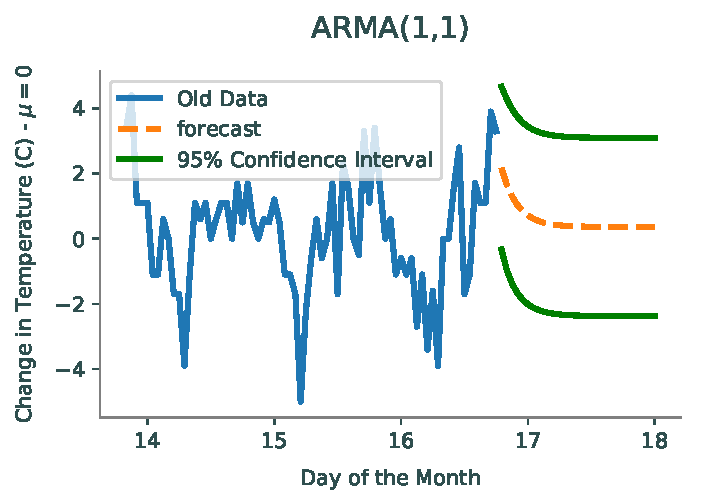
\includegraphics[width=\textwidth]{figures/arma.pdf}
\caption{ARMA(1,1) forecast on \li{weather.npy}}
\label{fig:forecasted}
\end{figure}

As in other problems, the data passed in should be the time series stationary.
The AIC of an ARMA model object is saved as the attribute \li{aic}.
Since the AIC is much faster to compute using \li{statsmodels}, model identification is much faster.
Once a model is chosen, the method \li{predict} will forecast $n$ observations, where $n$ is the number of known observations.
It will return the mean of each future observation.

\begin{lstlisting}
# Predict from the beginning of the model to 30 observations in the future
model.predict(start=0,end=len(data)+30)
\end{lstlisting}

\begin{problem}
Write a function \li{sm_arma()} that accepts a \li{file} containing a time series, maximum integer values for $p$ and $q$, and the number $n$ of values to predict.
Use \li{statsmodels} to perform model identification as in Problem \ref{prob:model-identification}, where the order of ARMA($i,j$) satisfies $1\leq i \leq p$ and $1 \leq j \leq q$.
Ensure the model is fit using the MLE.

Use the optimal model to predict $n$ future observations of the time series.
Plot the original observations along with the mean of each future observations given by \li{statsmodels}.
Return the AIC of the optimal model.

For $p=3, q=3$, and $n=30$, your graph should look similar to Figure \ref{fig:sm}.  
How does this graph compare to Problem \ref{prob:naive}? Problem \ref{prob:arma:forecast}?
\label{prob:statsmodels}
\end{problem}

\begin{figure}[H]
\centering
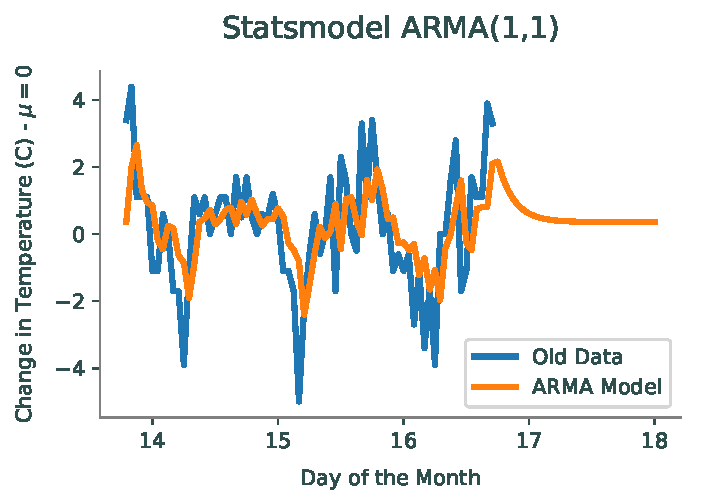
\includegraphics[width=\textwidth]{figures/sm.pdf}
\caption{Statsmodel ARMA(3,1) forecast on \li{weather.npy}.}
\label{fig:sm}
\end{figure}

The \li{ARMA} class can also perform model identification.
The method \li{arma_order_select_ic} will find the optimal order of the ARMA model based on certain criteria.
The first parameter \li{y} is the data.
The data must be a NumPy array, not a Pandas DataFrame.
The parameter \li{ic} defines the criteria trying to be minimized.
The method will return a dictionary, where the minimal order of each criteria can be accessed.
%\footnote{http://www.statsmodels.org/devel/generated/statsmodels.tsa.stattools.arma_order_select_ic.html}.

\begin{lstlisting}
>>> import statsmodel as sm
>>> from statsmodel.tsa.stattools import arma_order_select_ic as order_select
>>> import pandas as pd

>>> # Get sunspot data and give DateTimeIndex
>>> sunspot = sm.datasets.sunspots.load_pandas().data[['SUNACTIVITY']]
>>> sunspot.index = pd.Index(sm.tsa.datetools.dates_from_range('1700', '2008'))

>>> # Find best order where p < 5 and q < 5
>>> # Use AICc as basis for minimization
>>> order = order_select(sunspot.values,max_ar=4,max_ma=4,ic=['aic','bic'],fit_kw={'method':'mle'})
>>> print(order['aic_min_order'])
(4,2)
>>> print(order['bic_min_order'])
(4,2)
\end{lstlisting}

The method \li{plot_predict} accepts a time series and plots the ARMA model alongside the original data in a given range.
The plot of the ARMA model is the mean calculated by ARMA at each data point, both known and future.
This method works by giving a range on which to plot the ARMA model.
This range can be given by indices (as in Problem \ref{prob:statsmodels}) or by a DateTimeIndex.

\begin{lstlisting}
>>> # Fit model
>>> model = ARMA(dta, (4, 2)).fit(method='mle')

>>> # Create plot
>>> fig, ax = plt.subplots(figsize=(13,7))
>>> # Plot from 1950 to 2012. 
>>> fig = model.plot_predict(start='1950', end='2012', ax=ax)

>>> ax.set_title('Sunspot Dataset')
>>> ax.set_xlabel('Year')
>>> ax.set_ylabel('Number of Sunspots')
>>> plt.show()
\end{lstlisting}

\begin{figure}[H]
\centering
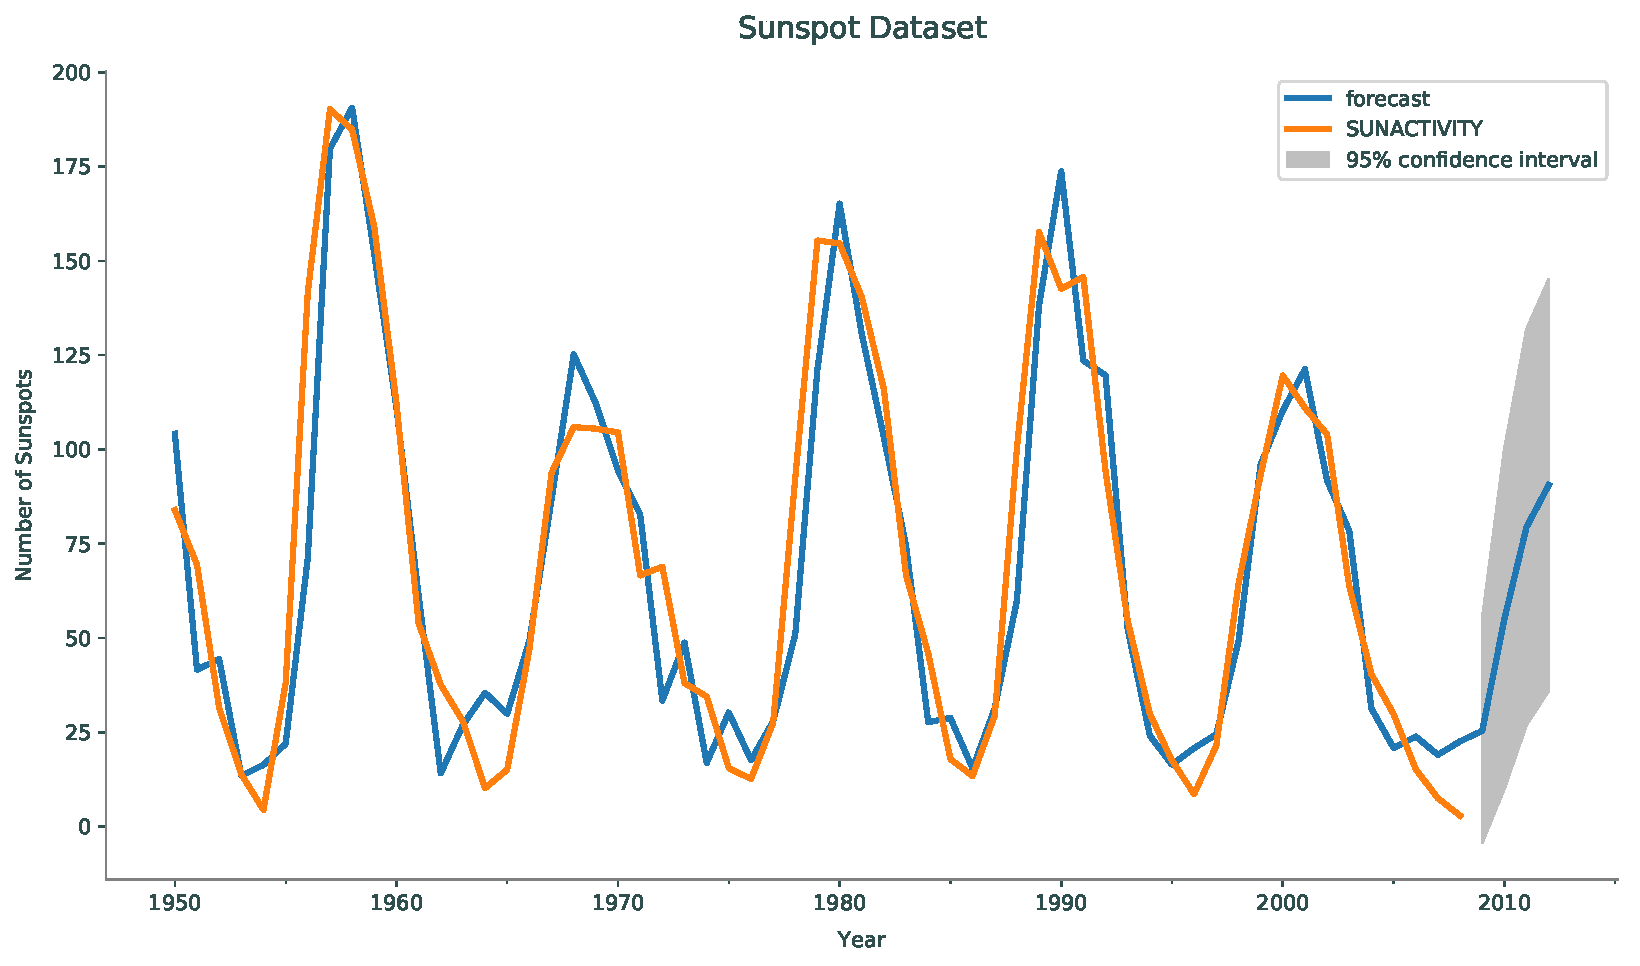
\includegraphics[width=\textwidth]{figures/sunspot.pdf}
\caption{Sunspot activity data is forecasted four years in the future using \li{statsmodels.}}
\label{fig:sunspot}
\end{figure}

\begin{problem}
The dataset \li{manaus} contains data on the height of the Rio Negro from every month between January 1903 and January 1993.
Write a function \li{manaus()} that accepts the forecasting range as strings \li{start} and \li{end}, the maximum parameter for the AR model \li{p} and the maximum parameter of the MA model \li{q}.
The parameters \li{start} and \li{end} should be strings corresponding to a DateTimeIndex in the form \li{Y\%M\%D}, where \li{D} is the last day of the month.

The function should determine the optimal order for the ARMA model based on the AIC and the BIC.
Then forecast and plot on the range given for both models and compare.
Return the order of the AIC model and the order of the BIC model, respectively.
For the range \li{'1983-01-31'} to \li{'1995-01-31'}, your plot should look like Figure \ref{fig:manaus}.

(Hint: The data passed into \li{arma_order_select_ic} must be a NumPy array. Use the attribute \li{values} of the Pandas DataFrame.)

To get the \li{manaus} dataset and set it with a DateTimeIndex, use the following code:
\begin{lstlisting}
>>> # Get dataset
>>> raw = pydata('manaus')
>>> # Convert to DateTimeIndex
>>> manaus = pd.DataFrame(raw.values,index=pd.date_range('1903-01','1993-01',freq='M'))
>>> manaus = manaus.drop(0,axis=1)
>>> # Set new column title
>>> manaus.columns = ['Water Level']
\end{lstlisting}
\label{prob:manaus}
\end{problem}

\begin{figure}[H]
\centering
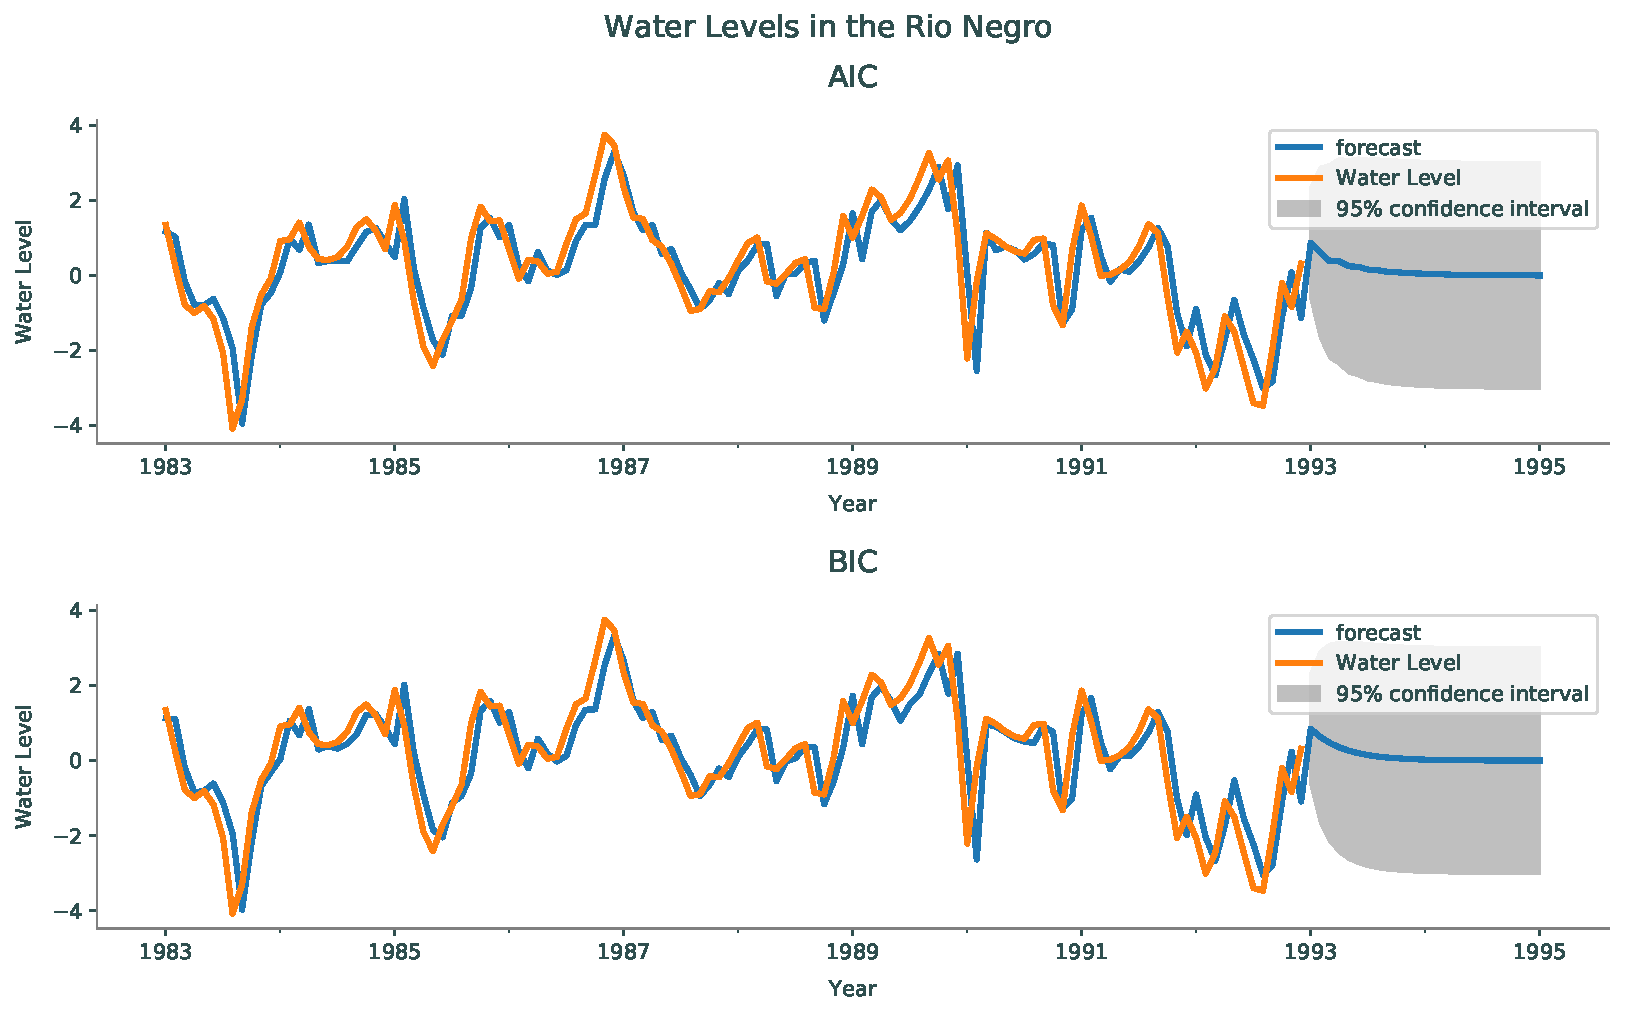
\includegraphics[width=\textwidth]{figures/manaus.pdf}
\caption{AIC and BIC based ARMA models of \li{manaus} dataset.}
\label{fig:manaus}
\end{figure}

% Additional Materials

\pagebreak

\section*{Additional Materials}

\subsection*{Finding Error Correlation}
To find the correlation of the current error with past error, the noise of the data needs to be isolated.
Each data point $y_t$ can be decomposed as

\begin{equation}
y_t=T_t+S_t+R_t,
\end{equation}

where $T_t$ is the overall trend of the data, $S_t$ is a seasonal trend, and $R_t$ is noise in the data.
The overall trend is what the data tends to do as a whole, while the seasonal trend is what the data does repeatedly.
For example, if looking at airfare prices over a decade, the overall trend of the data might be increasing due to inflation.
However, we can break this data into individual years.
We call each year a season.
The seasonal trend of the data might not be strictly increasing, but have increases during busy seasons such as Christmas and summer vacations.

To find $T_t$, we use an $M$-fold method.
In this case, $M$ is the length of our season.
We define the equation

\begin{equation}
T_t=\frac{1}{M}\sum_{-M/2<i<M/2}y_{i+t}.
\end{equation}

This means for each $t$, we take the average of the season surrounding $y_t$.

To find the seasonal trend, first subtract the overall trend from the time series.
Define $x_t=y_t-T_t$.
The value of the seasonal trend can then be found by averaging each day of the season over every season.
For example, if the season was one year, we would find the average value on the first day of the year over all seasons, then the second, and so on.
Thus,

\begin{equation}
S_t=\frac{1}{K}\sum_{i\equiv t\text{ (mod $M$)}}x_i
\end{equation}
where $K$ is the number of seasons.

With the overall and seasonal trend known, the noise of the data is simply $R_t=y_t-T_t-S_t$.
To determine the strength of correlations with the current error and the past error, plot $y_t$ vs. $R_{t-i}$ as in Figure \ref{fig:correlations}.

\subsection*{Proof of Equation \ref{eq:update-z}} 
\begin{align}
    \sum_{i=1}^p\phi_i(z_{t-i}-\mu)+a_t+\sum_{j=1}^q\theta_ja_{t-j}&=\sum_{i=1}^p\phi_i(H\hat{\textbf{x}}_{t-i})+a_t+\sum_{j=1}^q\theta_ja_{t-j}\\
    &=\sum_{i=1}^r\phi_i(x_{t-i}+\sum_{k=1}^{r-1}\theta_kx_{t-i-k})+a_t+\sum_{j=1}^{r-1}\theta_ja_{t-j}\\
    &=a_t+\sum_{i=1}^r\phi_i(x_{t-i})+\sum_{j=1}^{r-1}\theta_j\Bigl(\sum_{i=1}^r\phi_ix_{t-j-i}+a_{t-j}\Bigr)\\
    &=a_t+\sum_{i=1}^r\phi_i(x_{t-i})+\sum_{j=1}^{r-1}\theta_jx_{t-k}\\
    &=x_t+\sum_{j=1}^{r-1}\theta_jx_{t-k}\theta_kx_{t-k}\\
    &=z_t.
\end{align}

%%%%%%%%%%%%%%%%%%%%%%%%%%%%%%%%%%%%%%